\documentclass[conference]{IEEEtran}
\IEEEoverridecommandlockouts

\usepackage{cite}
\usepackage{amsmath}
\usepackage{amssymb}
\usepackage{amsfonts}
\usepackage{graphicx}
\usepackage{booktabs}
\usepackage{tikz}
\usepackage{textcomp}
\usepackage{url}
\usepackage{hyperref}

\hypersetup{
    colorlinks=false,
    pdfborder={0 0 0},
    pdftitle={AutoOps AI: An Explicit Multi-Agent State-Machine Framework for Closed-Loop, Risk-Gated Infrastructure Remediation},
    pdfauthor={}
}

% Tighten float/caption spacing; at IEEEtran defaults the whitespace around
% this paper's floats runs to most of a column.
\setlength{\textfloatsep}{6pt plus 2pt minus 2pt}
\setlength{\floatsep}{6pt plus 2pt minus 2pt}
\setlength{\intextsep}{6pt plus 2pt minus 2pt}
\setlength{\dbltextfloatsep}{6pt plus 2pt minus 2pt}
\setlength{\abovecaptionskip}{3pt}
\setlength{\belowcaptionskip}{0pt}

\begin{document}

\title{AutoOps AI: An Explicit Multi-Agent State-Machine Framework for Closed-Loop, Risk-Gated Infrastructure Remediation}

\author{
  \begingroup
  \renewcommand{\arraystretch}{0.85}
  \begin{tabular}[t]{c@{\extracolsep{4em}}c}
    \normalsize Reina Mercy R & \normalsize Rahul Ramamoorthy \\[-0.4ex]
    \footnotesize\itshape UG Scholar & \footnotesize\itshape UG Scholar \\[-0.4ex]
    \footnotesize\itshape Dept. of Computer Science and Eng. & \footnotesize\itshape Dept. of Computer Science and Eng. \\[-0.4ex]
    \footnotesize\itshape Chennai Institute of Technology & \footnotesize\itshape Chennai Institute of Technology \\[-0.4ex]
    \footnotesize Chennai, India & \footnotesize Chennai, India \\[-0.4ex]
    \footnotesize reinamercyr.cse2023@citchennai.net & \footnotesize rahulramamoorthy.cse2023@citchennai.net \\[1.5ex]
    \normalsize Sathika Begum M & \normalsize Sankari S \\[-0.4ex]
    \footnotesize\itshape UG Scholar & \footnotesize\itshape Assistant Professor \\[-0.4ex]
    \footnotesize\itshape Dept. of Computer Science and Eng. & \footnotesize\itshape Dept. of Computer Science and Eng. \\[-0.4ex]
    \footnotesize\itshape Chennai Institute of Technology & \footnotesize\itshape Chennai Institute of Technology \\[-0.4ex]
    \footnotesize Chennai, India & \footnotesize Chennai, India \\[-0.4ex]
    \footnotesize sathikabegumm.cse2023@citchennai.net & \footnotesize sankaris@citchennai.net
  \end{tabular}
  \endgroup
}

\maketitle

\begin{abstract}
Detecting infrastructure failures is mature; diagnosing, fixing and
safely executing a remediation remains manual. AutoOps AI is a
closed-loop multi-agent framework whose risk-scoring engine routes every
generated plan to autonomous execution, notification or a human approval
gate, behind an independent command-pattern check no approval can
override. We test whether it generalizes remediation \emph{planning} to
five incident classes held out from its remediation knowledge (though
detectable by predefined signatures), scoring plan \emph{content}
against a per-class rubric because a simulated executor's success flag
is independent of plan quality. Scoring \emph{containment} of a required
action rewards verbosity: a length-matched random planner scores 58.8\%.
Requiring a correct action \emph{and} no irrelevant one, the full system
reaches \textbf{47.0\%} intent-to-treat (95\% CI 37.5--56.7; 50.5\% over
the 93 incidents where the model produced a usable plan) against
\textbf{4.3\%} for that control (incident-level Monte Carlo null,
$p\approx5.0\times10^{-5}$), at $4.1\times$ the median latency; a
rule-based arm scores 0.0\% by construction. On covered classes the full
and rule-based arms score identically (66.7\%), concealing a regression
on one class, a matching gain on another, and a memory cache replicating
correct and incorrect fixes alike. Content-aware scoring also exposed
non-dispatchable template actions, a source-attribution bug, and a risk
score whose dominant inputs are self-reported by the planner and
saturate its range. Retrieval contributed nothing to the held-out
experiment and remains untested. All results use
\texttt{openai/gpt-oss-120b}.
\end{abstract}

\begin{IEEEkeywords}
AIOps, multi-agent systems, large language models, incident response,
risk-based decision routing, empirical evaluation
\end{IEEEkeywords}

\section{Introduction}

Observability tooling has matured; diagnosis and remediation have not.
Correlating an alert with a root cause, judging whether a fix is safe,
and executing it remain manual. LLMs with chain-of-thought~\cite{cot} and
tool use~\cite{react} can select actions from a constrained tool
surface, and retrieval~\cite{rag-lewis} can ground them in context, but
wiring a model to a control plane is unacceptable without safeguards: a
hallucinated \texttt{kubectl delete namespace} is not recoverable.
AutoOps AI therefore combines \textbf{command-level safety} ---
validating every step against hard-blocked patterns, independent of
planner confidence --- with \textbf{risk-proportional oversight}, which
escalates from autonomous execution through notification to human
approval as estimated risk rises. The first a human cannot override;
the second they can.

Contributions, ordered by strength of evidence: (i)~a controlled
\textbf{generalization experiment} on five classes held out from
remediation (not detection) knowledge, scored on plan content with a
length-matched random control; (ii)~evidence that \textbf{containment
scoring is unsound}, with a precision-aware measure and an
incident-level Monte Carlo null replacing a pooled random sample treated
as a second arm; (iii)~a \textbf{measured planning cascade} whose
per-class decomposition reverses its numerically identical aggregate;
and (iv)~\textbf{failure modes exposed by content-aware evaluation},
including non-dispatchable actions, a saturating self-reported risk
score, and a cold-start protocol that left retrieval untested.

\section{Related Work}

Most AIOps work addresses detection rather than
remediation~\cite{aiops-survey,aiops-llm-survey}, and TraceDiag shows
efficiency is often the harder production problem~\cite{tracediag}.
RCACopilot~\cite{rcacopilot} produces a root-cause diagnosis, not an
executed fix; Sarda et al.~\cite{sarda-autoremediation} let an LLM
propose and apply microservice remediations without a risk gate.
STRATUS~\cite{stratus}, the closest relative, is a multi-agent state
machine enforcing a formal \emph{Transactional No-Regression} property,
and AIOpsLab~\cite{aiopslab} benchmarks agents across the
detection-to-mitigation lifecycle. AutoOps AI differs in making the model
the \emph{least}-preferred of four plan sources under a graded rather
than binary safety gate, and its evaluation scores plan content on
held-out classes where these systems report outcome metrics.
RAG4ITOps~\cite{rag4itops} fine-tunes a retriever for IT-operations
text; we use an off-the-shelf embedding model,
\texttt{all-MiniLM-L6-v2}~\cite{sbert}. Kubernetes operators reconcile
toward a declared state~\cite{borg-omega-k8s} but need a hand-written
rule per failure mode, the role AutoOps AI's template layer plays.

\section{System Architecture}

AutoOps AI has four layers (Fig.~\ref{fig:architecture}): ingestion,
storage, a six-agent pipeline, and an interface. Each incident is one
JSON-serializable state object threaded through every agent; agents
return patched copies, giving a reconstructable decision history. Events
come from a simulator (used here) or a log ingester. Each storage backend
(relational store, cache, vector store, message bus, cluster client)
attempts a real connection at startup and otherwise substitutes an
in-process equivalent behind the same interface.

\begin{figure}[t]
\centering
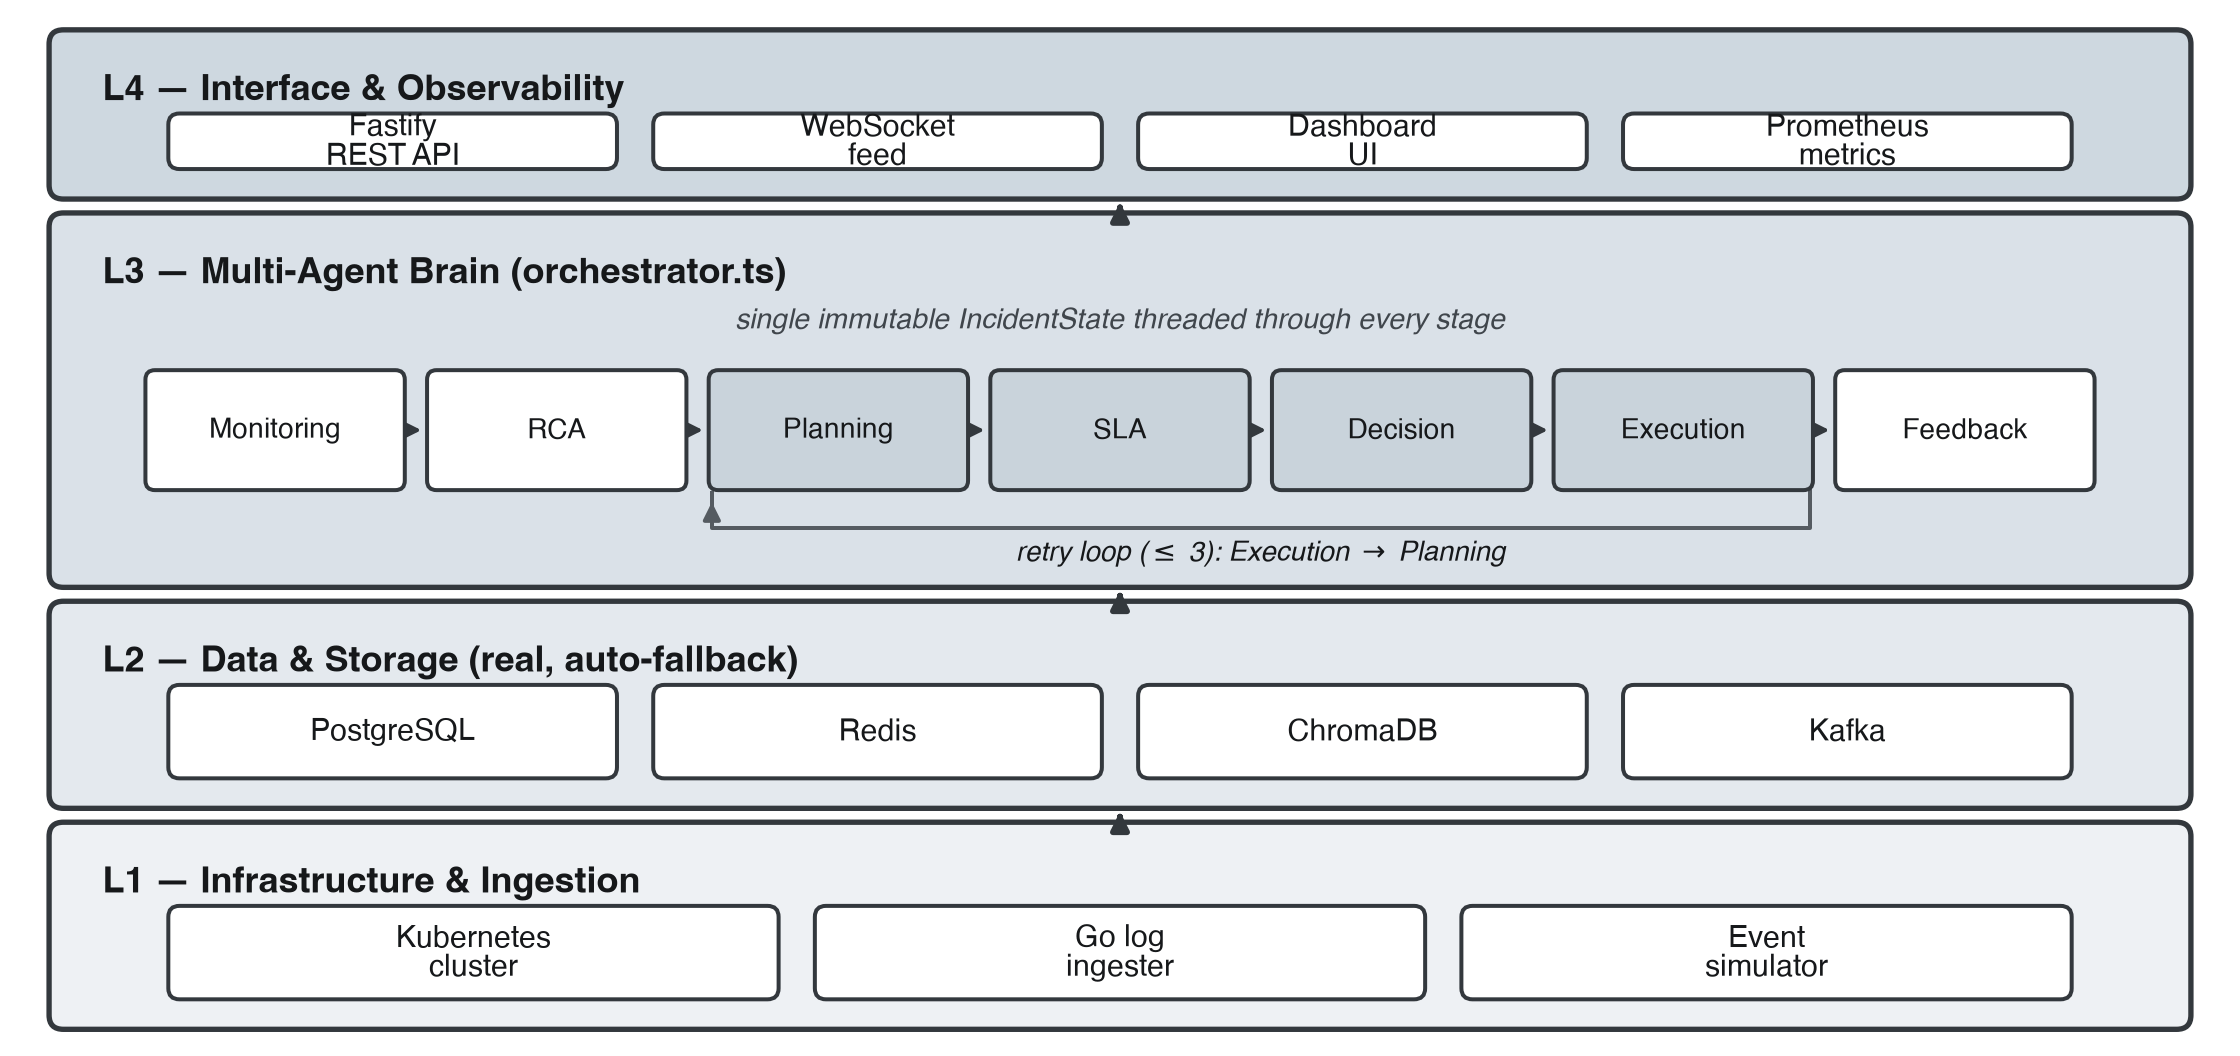
\includegraphics[width=0.62\linewidth]{figures/architecture.png}
\caption{AutoOps AI's four-layer architecture and bounded retry loop.}
\label{fig:architecture}
\end{figure}

\textbf{Monitoring} raises an incident when the anomaly score
$A = 0.3S + 0.4P + 0.3R$ (statistical, signature-pattern and clustering
sub-scores) reaches 0.7; the pattern set includes signatures for the
held-out classes (Section~\ref{sec:heldoutdef}). Incident type resolves
by a priority chain over matched event types, not by majority, a
property behind one defect in Section~\ref{sec:defects}. \textbf{RCA}
matches seven hand-authored rules and traces blast radius through a
static 13-node dependency graph. \textbf{Planning} tries, in order:
(1)~a \textbf{template} (confidence 0.95); (2)~\textbf{memory}, a past
fix at similarity $\geq0.82$, via a short-TTL fingerprint cache falling
through to vector search; (3)~the \textbf{language model}, prompted with
the top-3 similar past incidents; (4)~a per-category hardcoded
\textbf{fallback} if the model call fails or its output is unparseable.
Memory is skipped for unresponsive-service incidents.

\textbf{Decision Engine.} Every plan is re-validated against hard-block
and require-review patterns, then scored $\mathcal{R}\in[0,100]$:
\begin{equation}
\begin{aligned}
\mathcal{R} = \ & 20\,b + 30(1-c) + 15\cdot\mathbb{1}[\sigma=\texttt{crit}] \\
& - 20\cdot\mathbb{1}[\mathrm{rollback}] - 25\cdot\mathbb{1}[\sigma_{\mathrm{src}}=\texttt{tmpl}] \\
& - 15\cdot\mathbb{1}[\mathrm{trust}] - 5\cdot\mathbb{1}[\mathrm{memHit}\wedge\neg\mathrm{trust}]
\end{aligned}
\label{eq:risk}
\end{equation}
($b$ blast radius, $c$ confidence, $\sigma$ severity, $\mathrm{trust}$ a
memory fix with $\geq3$ successes), clamped and tiered: \texttt{auto}
below 35, \texttt{notify} to 65, \texttt{approve} to 85, \texttt{block}
above; templates are capped at \texttt{notify}. \texttt{auto} executes;
\texttt{notify} executes and notifies; \texttt{approve} and
\texttt{block} both suspend for a human decision and execute if it is
granted.

\textbf{Two gates with different authority.} The \texttt{block} tier is
an overridable approval gate, differing from \texttt{approve} only in the
score that reached it. The unconditional refusal is separate: the
command-pattern check (namespace deletion, unscoped destructive SQL,
shell-into-pod, pipe-to-shell) re-runs inside the Execution agent after
any approval and rejects the plan outright. A human can approve a
maximum-risk plan into execution, but not a hard-blocked command.

\textbf{$b$ and $c$ are not independent measurements.} Both derive from
the planner's own \texttt{riskLevel}: \texttt{critical} maps to
$b{=}5, c{=}0.5$, \texttt{high} to $b{=}3, c{=}0.5$, otherwise $b{=}2$,
$c\in\{0.7,0.9\}$. The model being assessed thus supplies the two
dominant inputs to its own score. At $b{=}5$ the blast term alone
contributes 100 before the remaining terms are added; in the held-out
data the resulting raw score was 110, then clamped to 100. This
saturation makes several other terms ineffective at changing the routed
tier for these incidents, although they still contribute to the
pre-clamp score. Eq.~\eqref{eq:risk} is a heuristic routing score, not a
calibrated risk estimate (Section~\ref{sec:riskgate}).

\textbf{Execution} runs steps in order, halting on first failure; four of
ten actions use a real Kubernetes client when one is reachable, six
always simulate, and dispatch switches on the action name.
\textbf{Feedback} persists the outcome and updates a memory fix's score
$s'=0.7s+0.3r$ ($r{=}1.0$ on success, lower otherwise); three successes
make a fix \emph{trustworthy}, tripling
its risk discount. Planning, risk scoring and execution loop under a
retry limit, re-planning with the failure as context; plans with zero or
implausibly many steps are rejected.

\section{Experimental Evaluation}

\subsection{Setup and Plan-Quality Measure}
\textbf{Experiment~1} (primary) tests generalization of remediation
planning to five held-out classes; \textbf{Experiment~2} characterizes
the cascade on the six covered classes. Both run the live pipeline in
simulate mode with the model at low temperature in JSON mode. All
figures use \texttt{openai/gpt-oss-120b}; an earlier version used
\texttt{llama-3.3-70b-versatile}, which its provider retired mid-study,
and every result was regenerated rather than mixed, with the superseded
run retained in the released artifacts. The replacement is a reasoning
model, which changed latency and token cost but not the protocol.

The simulated executor fails each step on an independent random draw
regardless of what it says, so resolution rate cannot separate a sound
plan from a generic one. The primary measure is therefore \textbf{plan
correctness}, scored from content against a rubric fixed in advance:
per class, required actions and the wider set with a defensible role.
Our first measure, \textbf{containment} (any required action present),
is unsound: generated plans average 5.0 actions against the rule-based
arm's 2.00, and a five-action plan hits a given action about half the
time by chance. A \textbf{length-matched random planner} (uniform draws
without replacement at each incident's observed plan length) scores
\textbf{58.8\%} on containment. The primary \textbf{strict} measure
requires a required action \emph{and} no action outside the defensible
set; the random control falls to 4.3\%. Extra relevant steps are not
penalized, and read-only diagnostics are excluded from the precision
denominator. For significance we use an \textbf{incident-level Monte
Carlo null} rather than the pooled random sample: one length-matched
random plan per real incident, the whole $n$-incident experiment scored
and repeated, giving the distribution of totals chance produces at this
sample size. Table~\ref{tab:rubric} gives the held-out rubric in full so
every figure can be recomputed from the released plans.

\begin{table}[htbp]
\caption{Held-out rubric. \textbf{Req.}: at least one necessary.
\textbf{Defensible}: permitted, not sufficient. \textbf{Irrelevant}: any
occurrence fails the strict measure. cfg~=~\texttt{apply\_config},
pipe~=~\texttt{trigger\_pipeline},
lim~=~\texttt{update\_resource\_limits},
pool~=~\texttt{flush\_connection\_pool},
rbk~=~\texttt{rollback\_deployment}, rst~=~\texttt{restart\_service},
roll~=~\texttt{rolling\_restart}, scl~=~\texttt{scale\_deployment},
hlth~=~\texttt{verify\_health}, disk~=~\texttt{clear\_disk\_space}.}
\label{tab:rubric}
\centering
\scriptsize\setlength{\tabcolsep}{4pt}
\renewcommand{\arraystretch}{0.9}
\begin{tabular}{@{}llll@{}}
\toprule
\textbf{Class} & \textbf{Req.} & \textbf{Defensible} & \textbf{Irrelevant} \\
\midrule
\texttt{cert\_expiry}    & cfg, pipe & roll, rst, hlth, scl      & rbk, lim, disk, pool \\
\texttt{dns\_failure}$^{\ast}$ & cfg  & rst, roll, hlth, scl      & rbk, lim, disk, pool, pipe \\
\texttt{config\_drift}   & cfg, rbk  & roll, rst, hlth, pipe, scl & lim, disk, pool \\
\texttt{cpu\_throttling} & lim       & cfg, roll, hlth, scl      & rst, rbk, disk, pool, pipe \\
\texttt{db\_deadlock}    & pool      & rst, roll, cfg, hlth      & scl, rbk, lim, disk, pipe \\
\bottomrule
\multicolumn{4}{p{8.2cm}}{\scriptsize $^{\ast}$Also admits
\texttt{restart\_service} as sufficient when the step targets the
resolver (\texttt{dns}, \texttt{coredns}, \texttt{kube-dns},
\texttt{resolver}) rather than the application --- the rubric's one
content-sensitive clause.} \\
\end{tabular}
\renewcommand{\arraystretch}{1}
\end{table}

\label{sec:rubricthreats}
The rubric is author-defined and we scored our own system. It was fixed
before the experiments and kept lenient toward the baseline, and it
discriminates as intended: the generic fallback fails all five held-out
classes, hand-written plans pass all five, and the baseline passes
covered classes with a runbook. One post-hoc correction --- admitting an
equivalent restart action for a template-handled covered class ---
favoured the baseline. The rubric is versioned and every result file
records the version it was scored under. This is the study's principal
threat to validity (Section~\ref{sec:limits}).

\subsection{Protocol and Baseline}
\label{sec:heldout}
\label{sec:heldoutdef}
The five held-out classes --- expired TLS certificate, DNS resolution
failure, configuration drift, CPU throttling under a too-tight limit,
database deadlock --- have no template, stored fix or category-specific
fallback. They are held out from \emph{remediation}, not
\emph{detection}: each has a detection signature, as teams routinely
alert on failures they have no runbook for, and without one no incident
is raised in either arm. Signatures are identical across arms and affect
only whether an incident enters the pipeline, not its outcome.

The vector store and fix cache are cleared before every incident so that
late incidents cannot be served fixes learned from earlier ones; in a
preliminary run the first \texttt{dns\_failure} incident was served a
stored \texttt{cert\_expiry} plan across a similarity threshold
(Section~\ref{sec:defects}). Model-sourced plans earn no risk discount,
so most held-out incidents reached \texttt{approve} or \texttt{block} and
suspended; the harness acted as approving operator through the
production endpoint, so no routing logic was bypassed. Consequently
latency excludes human decision time, and every gated incident ---
including \texttt{block} --- was approved: resolution rates describe
permissive supervision and measure the pipeline downstream of the gate,
not the gate's value as a safety control.

The \textbf{rule-based baseline} is an evaluation-only flag skipping
memory and the model, routing every non-template incident to the same
hardcoded fallback; detection, RCA, risk scoring, execution and retry
are identical. Both arms receive byte-identical event content, so
comparisons between them are paired.

\subsection{Evaluation Integrity}
\label{sec:integrity}
An earlier version of this evaluation was invalidated by harness defects
(Section~\ref{sec:defects}), and provider quota exhaustion produced
class-correlated missing data. The current harness makes both failure
modes detectable from the released artifacts. \emph{Frozen assignment}:
a seeded permutation over all (class, run) pairs, with content derived
from (class, run index) rather than position. \emph{Arm and backend
verification}: results are refused if the server's arm disagrees with
the one claimed or any backend expected to be real reports an
in-process fallback. \emph{Per-call provenance}: provider-returned model
identifier and token counts. \emph{Quota pause}: exhaustion is
distinguished from transient rate limiting by the returned error. The
incident whose call triggers detection still records a fallback plan,
like any model-call failure; the \emph{harness} then stops issuing
further incidents, checkpoints, and later resumes at exactly those not
yet attempted, so exhaustion delays a run rather than degrading the rest
of it. \emph{Degradation guard}: a run whose model path falls back above
a fixed tolerance aborts. \emph{Artifacts}: source code, harness, seeded
work order, versioned rubric (\texttt{strict-1}), every per-incident
result file (superseded runs flagged) and the analysis scripts are at
\url{https://github.com/reinamercy/AutoOps}.

The labels \texttt{fallback} (a response that failed to parse after
retry) and \texttt{unavailable} (a call that failed outright: network
error, open circuit breaker, or quota exhaustion) differ only in cause;
both score the \emph{same} category-specific hardcoded plan, identical
to the rule-based arm's. Against the harness's exhaustion log, all 7
\texttt{unavailable} incidents in Experiment~1 and 5 of 6 in
Experiment~2 match a logged exhaustion event; the sixth
(\texttt{high\_error\_rate}) shows a 143-second call latency, an order of
magnitude above every other case, consistent with an unrelated transient
failure. Scoring is identical either way.

\begin{table}[htbp]
\caption{Held-out results ($n{=}20$/class, $N{=}100$/arm, paired;
random control $N{=}2000$, 20 draws at each observed plan length).}
\label{tab:heldout}
\centering
\scriptsize\setlength{\tabcolsep}{4pt}
\renewcommand{\arraystretch}{0.9}
\begin{tabular}{@{}lccc@{}}
\toprule
 & \textbf{AutoOps} & \textbf{Rule-based} & \textbf{Random} \\
\midrule
\multicolumn{4}{@{}l}{\emph{Strict plan correctness}} \\
\texttt{cert\_expiry}      & 15/20 & 0/20 & --- \\
\texttt{dns\_failure}      & 10/20 & 0/20 & --- \\
\texttt{config\_drift}     & 13/20 & 0/20 & --- \\
\texttt{cpu\_throttling}   & 9/20  & 0/20 & --- \\
\texttt{db\_deadlock}      & 0/20  & 0/20 & --- \\
\textbf{Overall}           & \textbf{47.0\%} & \textbf{0.0\%} & \textbf{4.3\%} \\
95\% CI                    & 37.5--56.7 & 0.0--3.7 & 3.5--5.3 \\
\midrule
Lenient (containment)      & 90.0\% & 0.0\% & 58.8\% \\
Mean action precision      & 0.876 & 0.900 & 0.565 \\
Median latency, ms         & 13{,}468 & 3{,}308 & --- \\
\quad IQR                  & 12{,}273--15{,}423 & 3{,}279--3{,}336 & --- \\
Mean latency, ms           & 15{,}196 & 3{,}443 & --- \\
\midrule
\multicolumn{4}{@{}l}{\emph{Risk-gate routing (Section~\ref{sec:riskgate})}} \\
\texttt{auto} (ungated)        & 0 & 0 & --- \\
\texttt{notify}                & 7 & 100 & --- \\
\texttt{approve} (human gate)  & 16 & 0 & --- \\
\texttt{block} (human gate)    & 77 & 0 & --- \\
Score at ceiling ($\mathcal{R}{=}100$) & 77 & 0 & --- \\
Distinct scores observed       & 3 & 1 & --- \\
Hard-blocked pattern fired     & 0 & 0 & --- \\
\bottomrule
\end{tabular}
\renewcommand{\arraystretch}{1}
\end{table}

\subsection{Experiment 1: Held-Out Classes}
Under the strict measure the full system reaches 47.0\% against the
rule-based floor of 0.0\% (Table~\ref{tab:heldout}). That comparison is
nearly vacuous, since no held-out class has a rule-based answer by
construction; the claim rests on the random control. Over $B{=}20{,}000$
replicates of the full 100-incident experiment, the length-matched
random planner's total has mean 3.7 (3.7\%), 95\% interval $[1,8]$, and
never exceeds 12 --- consistent with the pooled sample's 4.3\%, the
difference being sampling noise between estimates of the same rate
(2,000 against 2,000,000 draws). No replicate reaches the observed 47
($b{=}0$), so $p=(b+1)/(B+1)\approx5.0\times10^{-5}$, the smallest value
this many replicates resolve. Containment would report 90.0\% against
58.8\%, a 31-point margin; the strict measure gives 47.0\% against
4.3\%, a 43-point margin, because generated plans are precise (mean
0.876) and random ones are not (0.565).

Figures are \textbf{intent-to-treat}. Seven incidents lost the model call
to quota exhaustion and were scored on the hardcoded fallback, all
failures, so 47.0\% is the full system's rate, not the model's alone;
over the 93 with a usable model plan it is 47/93 = 50.5\%. The
interleaved order spread these losses over four classes
(\texttt{dns\_failure} 2, \texttt{config\_drift} 2,
\texttt{cpu\_throttling} 1, \texttt{db\_deadlock} 2, \texttt{cert\_expiry}
0) instead of concentrating them in whichever class ran last, the
confound that invalidated an earlier version of this table.
\texttt{db\_deadlock} reached the model on 18 of 20 incidents and scored
0/18, each pairing a right action with an irrelevant one --- below the
random planner's 1.2\% for this class, and a genuine class-level failure
rather than an artifact of ordering or sample size.

The advantage costs latency: median 13,468\,ms (IQR 12,273--15,423;
bootstrap 95\% CI for the median 12,909--13,980) against 3,308\,ms
(IQR 3,279--3,336), a $4.1\times$ ratio of medians. We compare medians
because the full arm is right-skewed: a 62.8-second maximum lifts its
mean to 15,196\,ms and the mean ratio to $4.4\times$.

McNemar's exact binomial test on discordant pairs --- not Fisher's
exact test, which assumes independent samples --- applies to all 100
pairs, none missing. On plan correctness 47 pairs favour the full system
and 0 the rule-based arm ($p<10^{-6}$). On resolution outcome there are
no discordant pairs: all 100 resolved in both arms. On the same pairs,
under the same simulator, the two metrics distinguish the arms very
differently --- the clearest evidence here that outcome and content
measure different things.

\label{sec:notshown}
\textbf{This experiment does not show retrieval works.} Clearing the
store before every incident leaves it empty at every generation call;
the record shows zero retrieved entries on all 93 model calls. Testing
retrieval needs a store warm on operational history yet cold on the
held-out classes; we built such a corpus from covered classes only, with
automated checks that no entry mentions a held-out class. We have
\emph{not} established that this works: a partial pilot under the
superseded model retrieved three entries on its first five incidents and
none on the remaining 35, for a reason not yet diagnosed. The ablation is
unrun, and we make no claim that retrieval helps, hurts or engages.

\subsection{Experiment 2: The Planning Cascade}
\label{sec:cascade}
On the six covered classes ($n{=}20$ each, $N{=}120$) plan sources are
template 60, memory 43, model 10, fallback 1, unavailable 6: the model
is reached on about one incident in twelve, and the two cheaper tiers
serve 86\% (Table~\ref{tab:covered}). Of the six incidents with no usable model plan, five
correspond to confirmed quota exhaustion and one to an unrelated
transient provider failure (Section~\ref{sec:integrity}); all six are
scored on the hardcoded fallback. Mean latency rises with tier: template
5,310\,ms, memory 6,491\,ms, model 13,754\,ms (single fallback
5,691\,ms), so templates complete $2.59\times$ faster than model plans
and cheapest-first ordering is a measured saving. Strict correctness by
source is 60/60, 14/43, 4/10, 0/1 and 2/6 respectively.

\begin{table}[htbp]
\caption{Strict correctness per covered class ($n{=}20$ each, paired).}
\label{tab:covered}
\centering
\scriptsize\setlength{\tabcolsep}{4pt}
\renewcommand{\arraystretch}{0.9}
\begin{tabular}{@{}lccc@{}}
\toprule
\textbf{Class} & \textbf{Full arm's sources} & \textbf{Full} & \textbf{Rule-based} \\
\midrule
\multicolumn{4}{@{}l}{\emph{Template-served in both arms --- identical by construction}} \\
\texttt{oom\_kill}     & template 20 & 20/20 & 20/20 \\
\texttt{cpu\_spike}    & template 20 & 20/20 & 20/20 \\
\texttt{service\_down} & template 20 & 20/20 & 20/20 \\
\midrule
\multicolumn{4}{@{}l}{\emph{No template --- the only classes where the arms can differ}} \\
\texttt{high\_error\_rate} & mem 14, LLM 4, unavail.\ 2 & \textbf{7/20} & \textbf{20/20} \\
\texttt{disk\_full}        & mem 14, LLM 2, fb 1, unavail.\ 3 & 0/20  & 0/20  \\
\texttt{conn\_pool\_exh.}  & mem 15, LLM 4, unavail.\ 1 & \textbf{13/20} & \textbf{0/20} \\
\midrule
\textbf{Non-template subtotal} & & \textbf{20/60} & \textbf{20/60} \\
\textbf{Overall}               & & 80/120 & 80/120 \\
\bottomrule
\end{tabular}
\renewcommand{\arraystretch}{1}
\end{table}

All comparisons are paired and use McNemar's exact test. In aggregate
both arms score 80/120 (66.7\%), with 13 discordant pairs each way and
94 concordant ($p=1.00$); on the 60 non-template incidents, the only
ones where the arms can differ, again 13 each way and 34 concordant
($p=1.00$). That tie conceals two opposing effects. On
\texttt{connection\_pool\_exhaustion} the generation path scores 13/20
against the fallback's 0/20, all 13 discordant pairs favouring it
($p=2.4\times10^{-4}$), because the fallback scales replicas instead of
recycling the pool; on \texttt{high\_error\_rate} it scores 7/20 against
20/20, all 13 discordant pairs favouring the rule-based arm
($p=2.4\times10^{-4}$) --- a \textbf{thirteen-incident regression against
a hardcoded default}. \texttt{disk\_full} is 0/20 in both arms (20
concordant pairs), a shared failure. The generation tiers produce
substantially different plans, not slower copies of the default, and
the null aggregate is two sizeable opposite effects cancelling.

\label{sec:amplify}
The regression traces mostly to memory, not the model. The cache serves
14 or 15 of 20 incidents per non-template class, but its fingerprint is
per-service, so several distinct fixes are cached per class, each
replicated across every later incident sharing that fingerprint with an
identical verdict. On \texttt{connection\_pool\_exhaustion} three of four
cached fixes are correct (9 incidents) and one wrong (6); on
\texttt{high\_error\_rate} two are correct (5) and two wrong (9); on
\texttt{disk\_full} all three are wrong (14). A class can therefore hold
a good and a bad cached fix at once, so gating admission on plan content
must happen per fingerprint. Under an executor whose outcomes are
independent of content, an incorrect replicated fix earns the tripled
\emph{trustworthy} discount of Eq.~\eqref{eq:risk} as readily as a
correct one, and correctness is never checked at storage. Model-sourced
plans reach 9/10 containment but only 4/10 strict, the imprecision
Experiment~1 found.

\subsection{Defects the Evaluation Exposed}
\label{sec:defects}
Scoring content rather than executor outcome surfaced five defects that
simulated execution had concealed.
\textbf{Non-dispatchable template actions.} Templates used descriptive
step labels the executor's fixed vocabulary did not recognize, so they
could not have run on a real cluster; the simulator reports success for
any action name, hiding it. The tier with the highest confidence,
largest risk discount and least oversight produced the least executable
plans. Aligning the vocabulary raised template correctness from 0/60 to
60/60. \textbf{Source attribution favoured the system.} An earlier build
labelled a plan model-sourced before the call and never reset it on
failure; with a stale model identifier making every call fail, the model
path in a prior report had not run at all. \textbf{Cross-class
retrieval.} A \texttt{dns\_failure} incident was served a stored
\texttt{cert\_expiry} plan: a threshold tuned on seen classes need not
discriminate unseen ones. \textbf{Order-dependent labelling.} Because
type resolves by priority, one filler event of another type relabelled
an entire incident, silently mislabelling a prior benchmark.
\textbf{A hand-set, saturating risk score.} Eq.~\eqref{eq:risk}'s
coefficients are not fitted to outcome data, and the blast term alone
contributes 100, the clamp value, for any plan labelled
\texttt{critical}.

\subsection{What the Risk Gate Actually Did}
\label{sec:riskgate}
Table~\ref{tab:heldout}'s lower block reports measured routing. No
held-out incident in either arm reached the ungated \texttt{auto} tier;
77 of the full arm's 100 sat at the score ceiling, only three distinct
scores occurred, and the hard-block check never fired. On Experiment~2's
covered classes, where most plans are template- or memory-sourced,
60.0\% (full) and 66.7\% (rule-based) reach \texttt{auto}. The full claim
is that held-out incidents received more human-gated routing than
covered ones. Whether 77\% warranted the highest tier this measurement
cannot answer: the score is heuristic, self-reported and saturating, and
those 77 incidents are the ones whose blast term contributed 100
because the planner labelled its own plan \texttt{critical}. This is a description of current behaviour, not
evidence the gate is calibrated.

\begin{figure}[!t]
\centering
% One-at-a-time term ablation of Eq. (1) -- Fig. 2.
% Bar values are read from risk_ablation_data.tex, which is generated by
%   npx tsx scripts/risk-decomposition.ts scripts/eval-heldout-full-gptoss120b.json \
%       --ablation-tex=../paper/figures/risk_ablation_data.tex
% Do not type values here.
% AUTO-GENERATED by autoops_ai/scripts/risk-decomposition.ts -- do not edit.
% Source: eval-heldout-full-gptoss120b.json (one-at-a-time term ablation of Eq. 1)
\def\ablationN{100}
\def\ablationRows{
  Blast radius/100,
  Severity/23,
  Confidence/16,
  Rollback/16,
  Template source/0,
  Trusted memory/0,
  Memory hit/0}
%
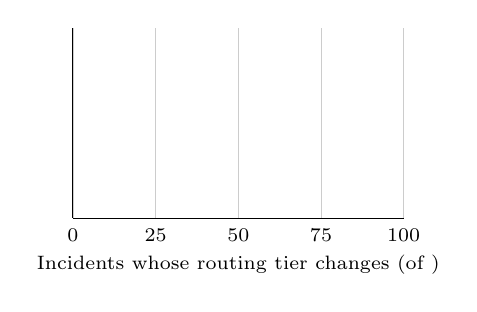
\begin{tikzpicture}[x=0.042cm, y=-0.34cm, font=\footnotesize]
  % gridlines and x axis
  \foreach \t in {0,25,50,75,100} {
    \draw[black!20, line width=0.3pt] (\t,0.45) -- (\t,7.55);
    \node[anchor=north, font=\scriptsize] at (\t,7.6) {\t};
  }
  \draw[line width=0.4pt] (0,7.55) -- (100,7.55);
  \node[anchor=north, font=\scriptsize] at (50,8.55)
    {Incidents whose routing tier changes (of \ablationN)};
  % bars with direct count labels
  \foreach \lab/\val [count=\i] in \ablationRows {
    \node[anchor=east] at (-1.5,\i) {\lab};
    \fill[black!60] (0,\i-0.3) rectangle (\val,\i+0.3);
    \node[anchor=west] at (\val+1,\i) {\val};
  }
  \draw[line width=0.4pt] (0,0.45) -- (0,7.55);
\end{tikzpicture}%

\caption{One-at-a-time sensitivity of Eq.~\eqref{eq:risk} on the 100
held-out incidents. Counts denote incidents whose routing tier changes
when the indicated term is removed; the planner-derived blast-radius
term is the dominant tier-determining component.}
\label{fig:riskablation}
\end{figure}

\textbf{Term ablation} (Fig.~\ref{fig:riskablation}).
Eq.~\eqref{eq:risk} reproduces all 100 recorded
full-arm scores. Raw scores took three values (44, 70, 110); the 77 at
110 clamp to 100, discarding 10 points. Zeroing one term at a time
changes the tier of 100/100 incidents for blast radius, 23 for severity,
16 for confidence and 16 for rollback; the template, trust and
memory-hit terms were zero on every held-out incident and change none.
For the 77 capped incidents, removing the $-20$ rollback discount does
not change the final score or tier, and removing severity or confidence
lowers the score without leaving \texttt{block}. In the rule-based arm (all 44), zeroing blast or severity
moves all 100 from \texttt{notify} to \texttt{auto}. Under one-at-a-time
ablation the planner-derived blast term is therefore the dominant
tier-determining input: the score is multi-factor in form but, on this
data, dominated in effect by one planner-supplied input.

\section{Discussion and Limitations}
\label{sec:limits}
Four actions were verified against a disposable cluster: dry-run left
state unmodified, and live mode produced a real rollout-restart
annotation, replica-count change and resource-limit patch. The other six
always simulate.

\textbf{Retrieval is untested.} The headline experiment measures a
language model, not retrieval-augmented planning
(Section~\ref{sec:notshown}); every retrieval claim here is
architectural.

\textbf{The rubric is author-defined and we scored our own system.} It
encodes our judgment, not production ground truth
(Section~\ref{sec:rubricthreats}), and has no independent validation;
ratings from practising SREs are the first thing we would add.

\textbf{No causal link between plan correctness and remediation.}
Executor outcomes are independent of plan content, so there is no
evidence a correct plan resolves anything: the paired test finds no
discordant pairs on resolution outcome against 47 on correctness. Only
four of ten actions were exercised against a real single-node cluster.
Establishing the link needs a fault-injection executor whose outcomes
depend on whether the injected fault was addressed.

\textbf{The hard block is not empirically evaluated.} No evaluated plan
triggered the unconditional command-pattern block, so this mechanism is
architecturally enforced but its empirical detection coverage is not
evaluated here.

\textbf{The learning loop is unguarded.} Memory caches and replicates
fixes regardless of correctness (Section~\ref{sec:amplify}) while
Eq.~\eqref{eq:risk} discounts risk for that tier, so the premise that a
reused fix is safer is unsupported by our data.

\textbf{Residual model-call loss.} Seven of 100 held-out incidents and
six of 120 covered incidents had no usable model plan (12 from quota
exhaustion, one transient); all are scored on the fallback rather than
excluded, and the interleaved order spread them across classes.

\textbf{Population and scale.} Eleven synthetic classes from one
author-written generator, $n{=}20$ per class; no external benchmark such
as AIOpsLab and no claim about production incident distributions.

\textbf{Undetected defects.} The model path in an earlier evaluation had
not run at all. Our answer is instrumentation, not assurance: plan
source, full plan content, arm verification and degradation guards are
retained for every run, so claims can be checked against raw records.

\section{Conclusion and Future Work}
On five classes it holds no remediation knowledge for, AutoOps AI's full
system produced a correct, precise plan in 47.0\% of 100 incidents
intent-to-treat (50.5\% where the model returned a usable plan), against
a 3.7\% chance null ($p\approx5.0\times10^{-5}$), at $4.1\times$ the median
latency; resolution outcome could not distinguish the arms at all. On
covered classes the full and rule-based arms tie exactly, hiding a gain
and a regression of thirteen incidents each. Methodologically,
containment scoring is unsound without a precision term and an
incident-level null; Eq.~\eqref{eq:risk}'s routing is dominated by one
planner-derived input on 77\% of held-out incidents; and clearing the store to
prevent memorization left retrieval untested. Future work, in order:
diagnose and run the retrieval ablation; replace the random-outcome
executor with fault injection; gate cache admission on content per
fingerprint; recalibrate the risk score; and obtain independent expert
ratings of the rubric.

{\scriptsize
\begin{thebibliography}{00}
\setlength{\itemsep}{0pt}
\setlength{\parskip}{0pt}
\bibitem{cot}
J. Wei \emph{et al.}, ``Chain-of-Thought Prompting Elicits Reasoning in
Large Language Models,'' \emph{NeurIPS}, vol. 35, 2022.

\bibitem{react}
S. Yao \emph{et al.}, ``ReAct: Synergizing Reasoning and Acting in
Language Models,'' \emph{ICLR}, 2023.

\bibitem{rag-lewis}
P. Lewis \emph{et al.}, ``Retrieval-Augmented Generation for
Knowledge-Intensive NLP Tasks,'' \emph{NeurIPS}, vol. 33, 2020.

\bibitem{aiops-survey}
M. Notaro, J. Cardoso, and M. Gerndt, ``A Systematic Mapping Study in
AIOps,'' \emph{arXiv:2012.09108}, 2020.

\bibitem{aiops-llm-survey}
L. Zhang \emph{et al.}, ``A Survey of AIOps in the Era of Large Language
Models,'' \emph{ACM Computing Surveys}, 2025.

\bibitem{tracediag}
R. Ding \emph{et al.}, ``TraceDiag: Adaptive, Interpretable, and
Efficient Root Cause Analysis on Large-Scale Microservice Systems,''
\emph{ESEC/FSE}, 2023.

\bibitem{rcacopilot}
Y. Chen \emph{et al.}, ``Automatic Root Cause Analysis via Large Language
Models for Cloud Incidents,'' \emph{EuroSys}, 2024.

\bibitem{sarda-autoremediation}
K. Sarda \emph{et al.}, ``Leveraging Large Language Models for the
Auto-Remediation of Microservice Applications,'' \emph{FSE Companion},
2024.

\bibitem{stratus}
Y. Chen \emph{et al.}, ``STRATUS: A Multi-Agent System for Autonomous
Reliability Engineering of Modern Clouds,'' \emph{NeurIPS}, 2025.

\bibitem{aiopslab}
Y. Chen \emph{et al.}, ``AIOpsLab: A Holistic Framework to Evaluate AI
Agents for Enabling Autonomous Clouds,'' \emph{MLSys}, 2025.

\bibitem{rag4itops}
T. Zhang \emph{et al.}, ``RAG4ITOps: A Supervised Fine-Tunable and
Comprehensive RAG Framework for IT Operations and Maintenance,''
\emph{EMNLP Industry Track}, 2024.

\bibitem{sbert}
N. Reimers and I. Gurevych, ``Sentence-BERT: Sentence Embeddings using
Siamese BERT-Networks,'' \emph{EMNLP}, 2019.

\bibitem{borg-omega-k8s}
B. Burns \emph{et al.}, ``Borg, Omega, and Kubernetes,'' \emph{ACM
Queue}, vol. 14, no. 1, 2016.

\end{thebibliography}
}

\end{document}
